% This file was converted to LaTeX by Writer2LaTeX ver. 1.4
% see http://writer2latex.sourceforge.net for more info
\documentclass[letterpaper]{article}
\usepackage[utf8]{inputenc}
\usepackage[T3,T1]{fontenc}
\usepackage[english]{babel}
\usepackage[noenc]{tipa}
\usepackage{tipx}
\usepackage[geometry,weather,misc,clock]{ifsym}
\usepackage{pifont}
\usepackage{eurosym}
\usepackage{amsmath}
\usepackage{wasysym}
\usepackage{amssymb,amsfonts,textcomp}
\usepackage{color}
\usepackage{array}
\usepackage{hhline}
\usepackage{hyperref}
\hypersetup{pdftex, colorlinks=true, linkcolor=blue, citecolor=blue, filecolor=blue, urlcolor=blue, pdftitle=}
\usepackage[pdftex]{graphicx}
% Page layout (geometry)
\setlength\voffset{-1in}
\setlength\hoffset{-1in}
\setlength\topmargin{20mm}
\setlength\oddsidemargin{20mm}
\setlength\textheight{239.4mm}
\setlength\textwidth{175.9mm}
\setlength\footskip{0.0cm}
\setlength\headheight{0cm}
\setlength\headsep{0cm}
% Footnote rule
\setlength{\skip\footins}{1.19mm}
\renewcommand\footnoterule{\vspace*{-0.18mm}\setlength\leftskip{0pt}\setlength\rightskip{0pt plus 1fil}\noindent\textcolor{black}{\rule{0.25\columnwidth}{0.18mm}}\vspace*{1.01mm}}
% Pages styles
\makeatletter
\newcommand\ps@Standard{
  \renewcommand\@oddhead{}
  \renewcommand\@evenhead{}
  \renewcommand\@oddfoot{}
  \renewcommand\@evenfoot{}
  \renewcommand\thepage{\arabic{page}}
}
\makeatother
\pagestyle{Standard}

\title{Image Analysis for Plant Communities}

\begin{document}
\maketitle

Notes for developing plant categorisation for bee-communities using image analysis and FIJI.

\section{Technology set-up and other stuff}
These are just a few notes for you to think about. Open source packages are ALWAYS more flexible because they are designed to be. It's good to familiarise yourself with them now if you can.

\subsection {Operating system}
Linux is much more reliable than Windows, if you can stretch yourself, then covert all your systems over. Linux comes in a range of 'flavours' but Ubuntu is a common distribution. Most stuff that works on Windows will work with Ubuntu (\url{http://www.ubuntu.com/}).

\subsection {WEB search engines}
Google does not seem as reliable as it
once was (e.g. see duckduck-go-6.pdf attached). Search results are less likely to be skewed with an engine like \textbf{DuckDuckGo }(DDG). Even better, you can be very specific about what you want with DDG \ by adding things like \ \textbf{f:pdf
'what ever your search is here'. } You can read more about it from the following sites:
\begin{enumerate}
\item {Syntax} \url{https://duck.co/help/results/syntax}
\item {Extras} \url{http://www.makeuseof.com/tag/6-really-cool-things-you-can-do-with-duckduckgo/}
\end{enumerate}

There are some other good search engines as well (e.g. Ixquick). Really, the key is to try and be flexible; get used to
using other types of search engines/ software and devices if you can? 

\subsection{Document processing}
When you have a lot of images in your document - then Latex is a much better option for writing up. It can be a little difficult to get you head around initially, but at the end of your write-up you will appreciate the effort. TeXstudio is a good platform (\url{http://www.texstudio.org/}). This document was written in TeXstudio, all the files are included in the subfolder tex-doc.

\subsection{Data entering/analysis and sharing}
Apache open office (entering data) and R-Studio (analysis) work well together - both integrate with TeXstudio. For example, you can export an Apache document (.odt) to a .tex file for opening in TeXstudio.

GitHub is an easy way to share large amounts of \emph{image} data online. You will need a repository manager. I used SmartGit, which has an easy to use desktop GUI. You can  manage you GitHub account (e.g. pushing and pulling information from you PC to the online GitHub account) and keep data synchronised.

\begin{enumerate}
\item Apache Open Office \url{http://www.openoffice.org/}
\item RStudio \url{https://www.rstudio.com/}
\item SmartGit \url{http://www.syntevo.com/smartgit/}
\end{enumerate}

\section{File and image data backup software}
Image files can be time consuming to back-up or copy, unless your using a good package. Grsync \label{Grsync} (\url{http://www.opbyte.it/grsync/}) is easy to use and once set up you can quickly synchronise data between drives.

\section{Select and download image management/pre-processing software}
Here are three. I tend to use XnView, especially for file management, naming, re-naming, cropping etc.


\begin{itemize}
\item XnView \url{http://www.xnview.com/en/} (see figure \ref{fig:1} below)
\item GIMP \url{http://www.gimp.org/}
\item InkScape \url{https://inkscape.org/en/}
\end{itemize}


\begin{figure}
\centering
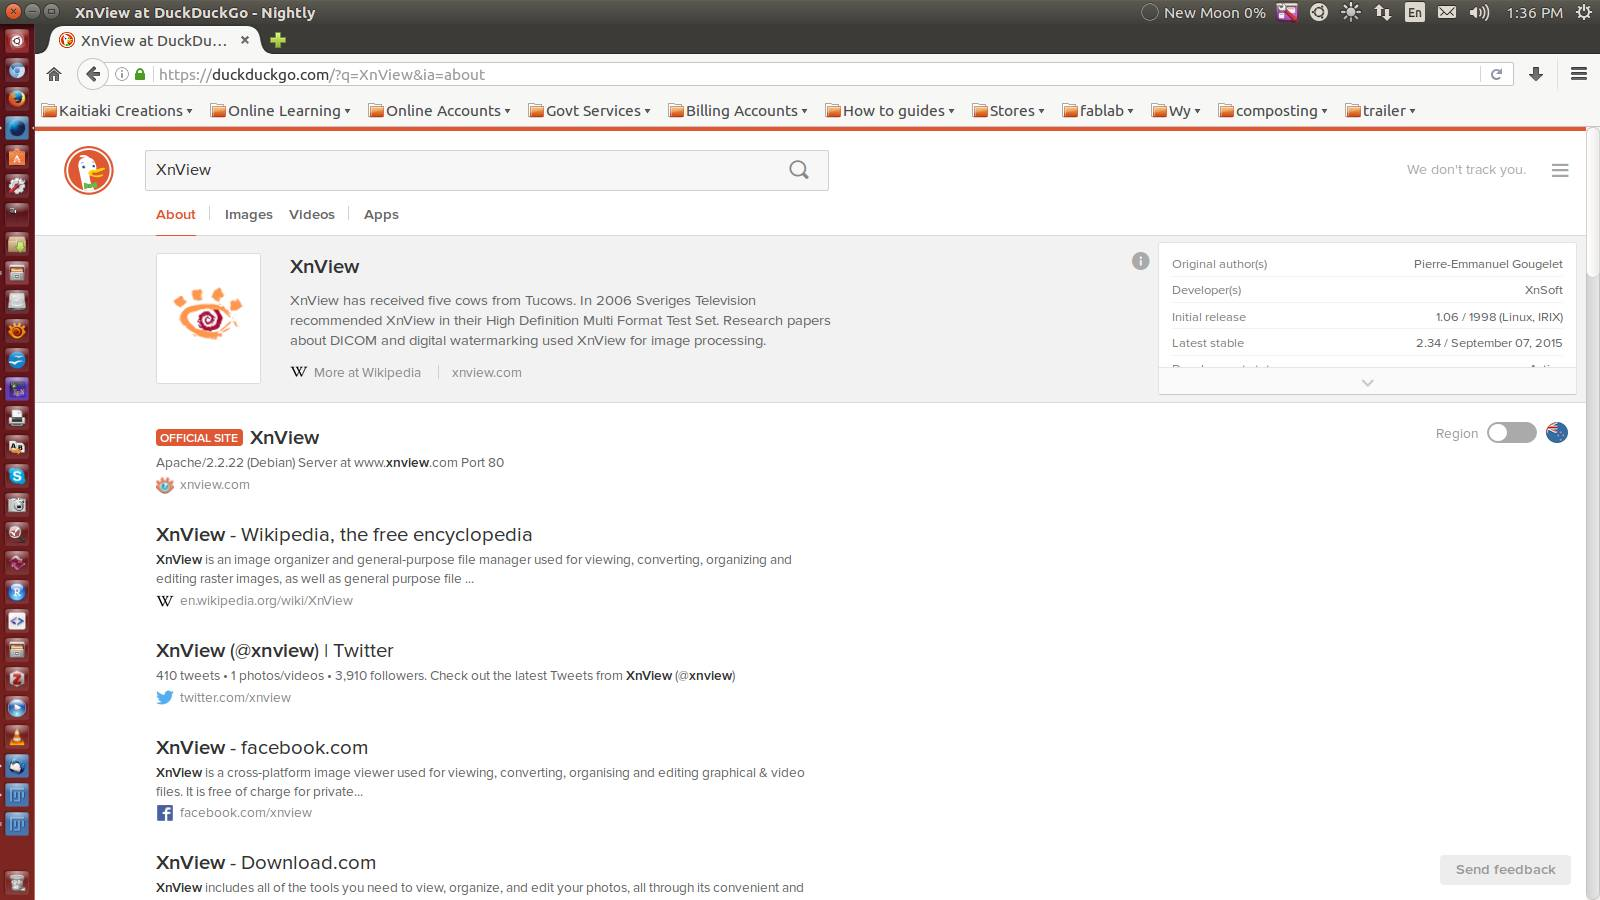
\includegraphics[width=175.9mm,height=98.94mm]{../e-tws/ddg} \caption{DuckDuckGo and XnView}\label{fig:1}
\end{figure}

\section{Download ImageJ/FIJI imaging software}
Download FIJI from here: \url{http://fiji.sc/Fiji}. Follow installation instructions.

\section{General image file handling procedures}
You won't need this if you only have a few image files. When processing images, data gets large quickly. It can be very difficult to manage properly; these are just some suggestions to help.
\begin{itemize}
\item Import raw image data.
\item If possible, save to 3x backups (e.g. 2x external HD, 1x internal partition disk) using Grsync (see section  section \ref{Grsync} above).
\item Set-up a \emph{working folder} structure. Try to anticipate some of the processing steps. Name the folders accordingly. For example, folder names could be: raw-images, sorted-date-location-images, rename, crop, normalise, segmented, etc...Once the structure has been decided, you can shorten the folder names.
\item Process a sample of images as per their folder ID -  complete an entire run of the processing cycle:
\subitem Step 1 FOLDER rename - rename files in Xnview.
\subitem Step 2 FOLDER crop - crop images to a grid.
\subitem Step 3 FOLDER normalise - set the saturation level of images.
\subitem Step 4 FOLDER segmented - classified images. See \autoref{sec:procedure-for-trainable-weka-segmentations-(tws)} below.
\subitem Step 5 FOLDER binary - convert classified images into binary images and post-process. 
\subitem Step 6 FOLDER analysis - count the number of, or assess the area of, target objects.
\item Repeat and refine the procedures. Check that results make sense.
\section {Verifying image analysis results.}
\item The most reliable/straightforward way to do this, is to manually estimate image  quantifications. For example, if you have counted five objects using the automatic classification method, then you should be able to count five objects in the images by manual inspection.
\end{itemize}

\section{Procedure for Trainable WEKA Segmentations (TWS)}\label{sec:procedure-for-trainable-weka-segmentations-(tws)}

\begin{enumerate}
\item Open FIJI.
\item Load image.
\begin{figure}[htps!]
\centering
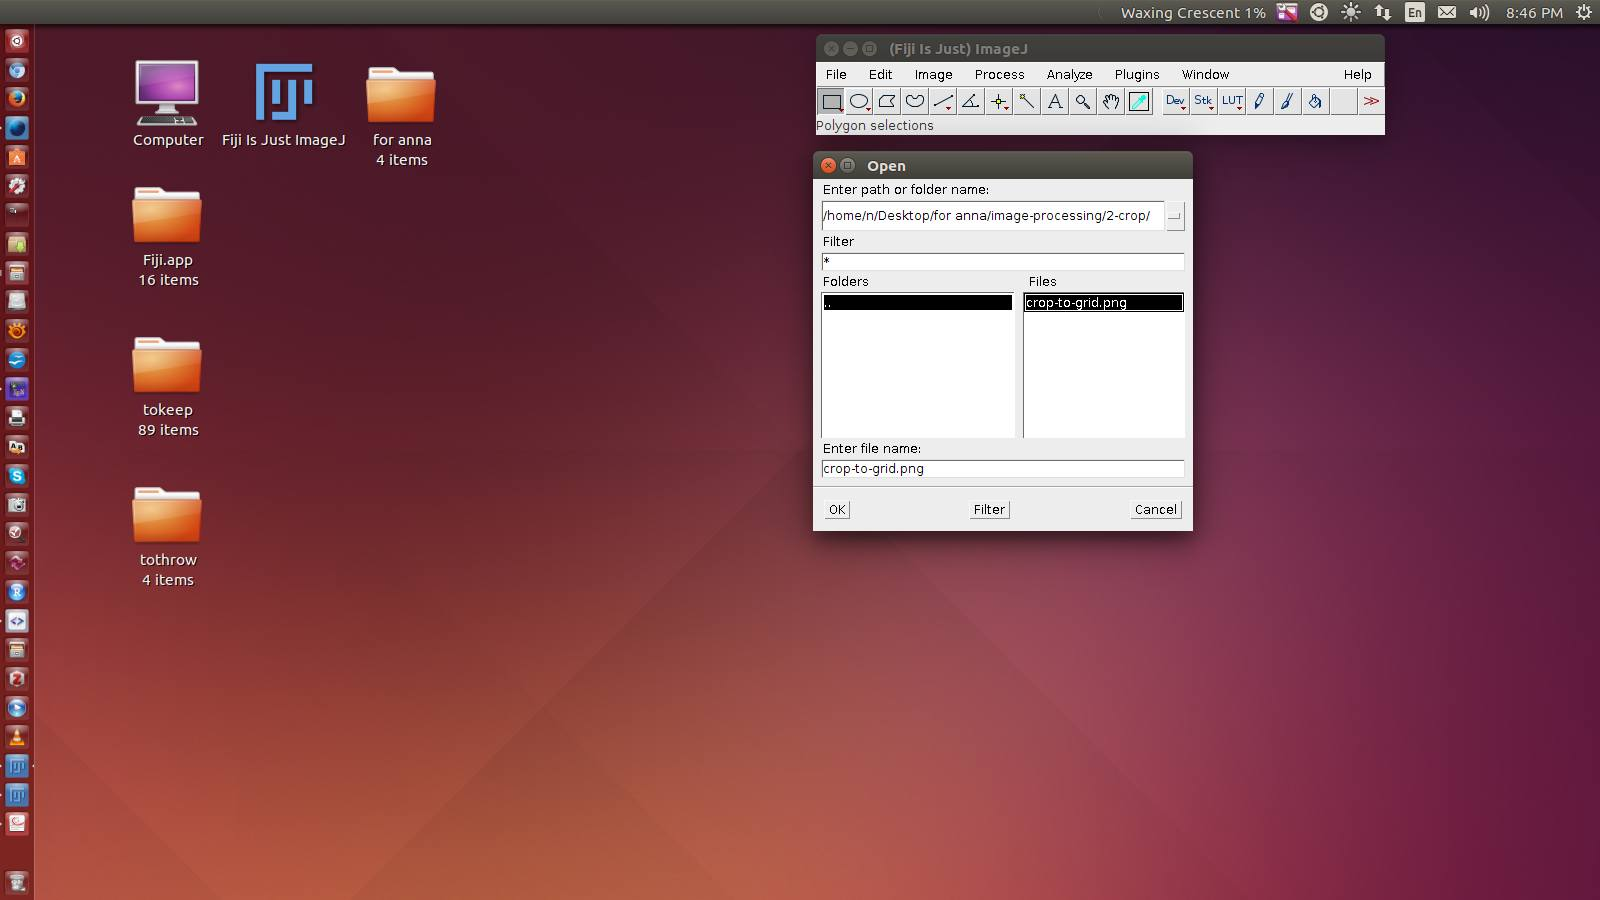
\includegraphics[width=0.7\linewidth]{../e-tws/1}
\caption{TWS Open file}
\label{fig:2}
\end{figure}
\clearpage

\item Load TWS plug-in.
\begin{figure}[htps!]
\centering
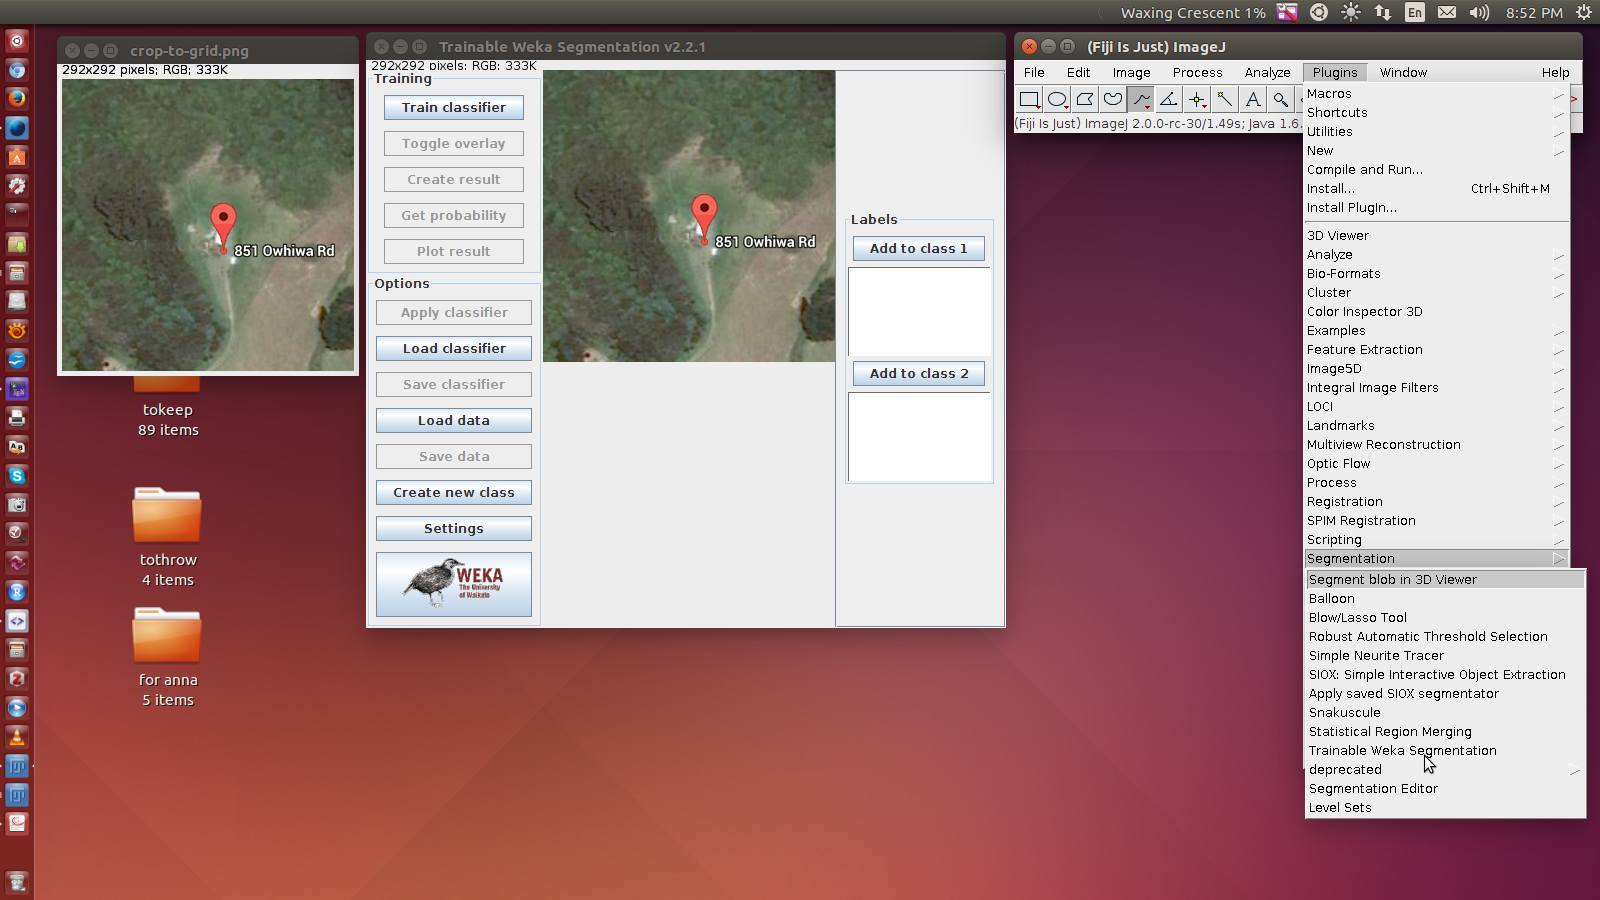
\includegraphics[width=0.7\linewidth]{../e-tws/2}
\caption{Load TWS plug-in.}
\label{fig:3}
\end{figure}

\item Set-up initial training.
\subitem A. De-select training features.
\subitem B. Set: Gaussian blur, Mean, Minimum, Maximum, Medium for initial runs.
\subitem C. Set Maximum sigma to 4.
\subitem D. Set Random Forest paramters to 50 trees, 7 random features.
\subitem E. For example, the Classifier options for this should now be:  hr.irb.fastRandomForest.FastRandomForest 
\subitem -I 50 -K 7 -S -188830655 -threads 2.

\begin{figure}[htps!]
\centering
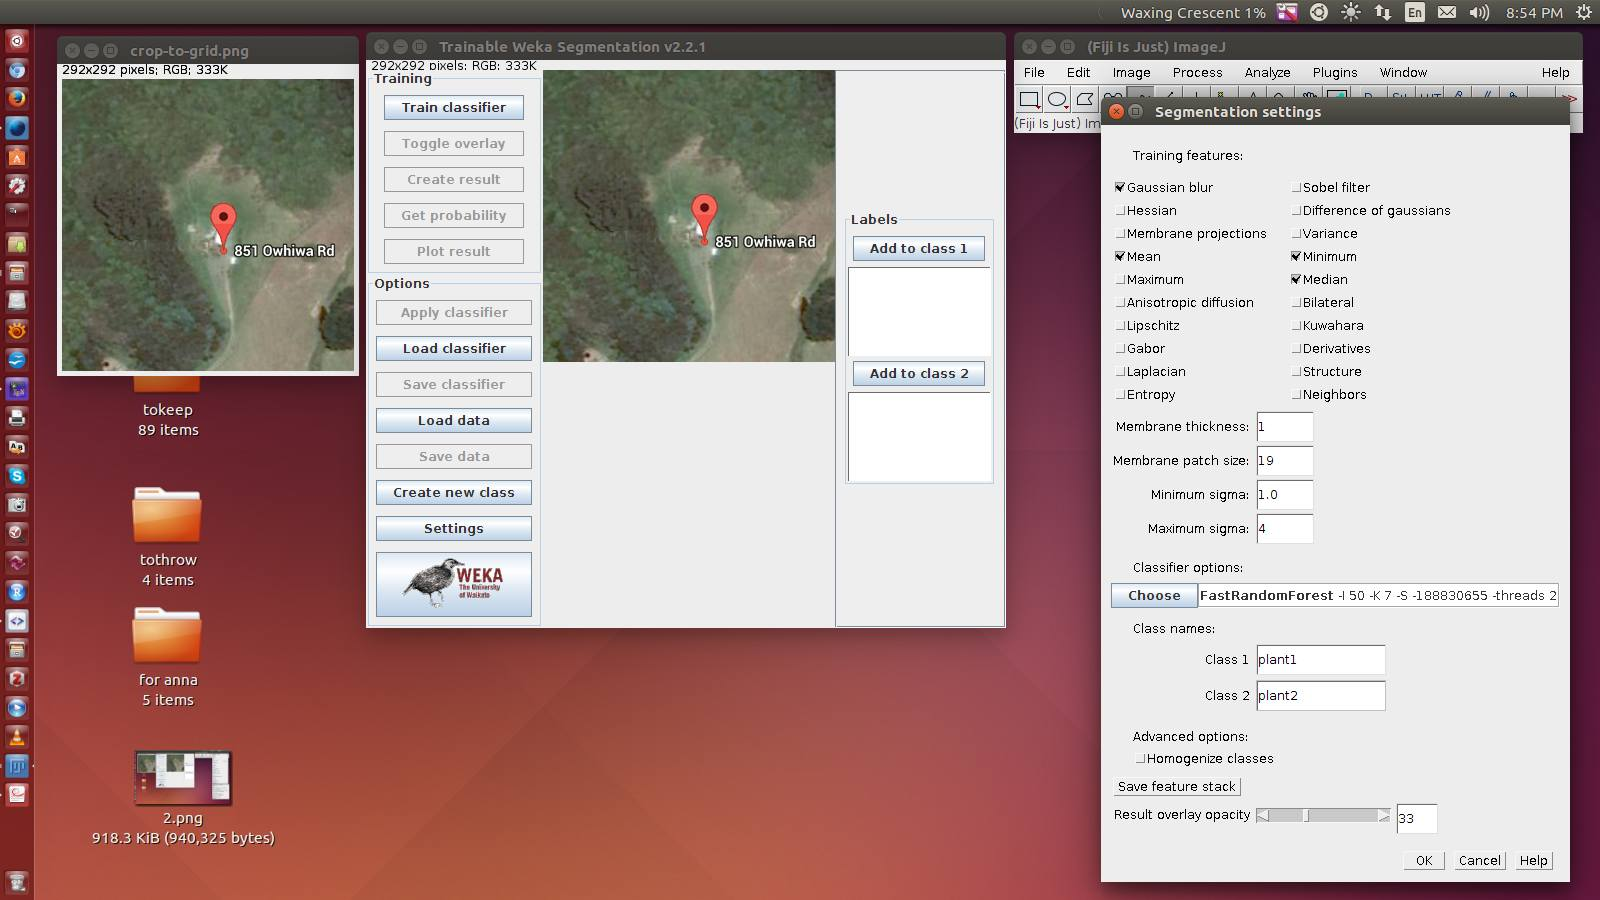
\includegraphics[width=0.7\linewidth]{../e-tws/3}
\caption{Set-up training and classifier parameters.}
\label{fig:4}
\end{figure}

\clearpage

\item Add more categories and supply trace samples.
\subitem A. There must be \emph{at least} one region of interest (RIO) example representing the target and background.
\subitem B. Use any of the ROI tools to add samples.
\subitem C. When providing ROI samples, LESS is more - the objective is to train the machine learner.
\subitem D. The algorithm needs to learn from a few \emph{key} samples. Otherwise, it is memorising your traces and \subitem regurgitating.

\begin{figure}[htps!]
\centering
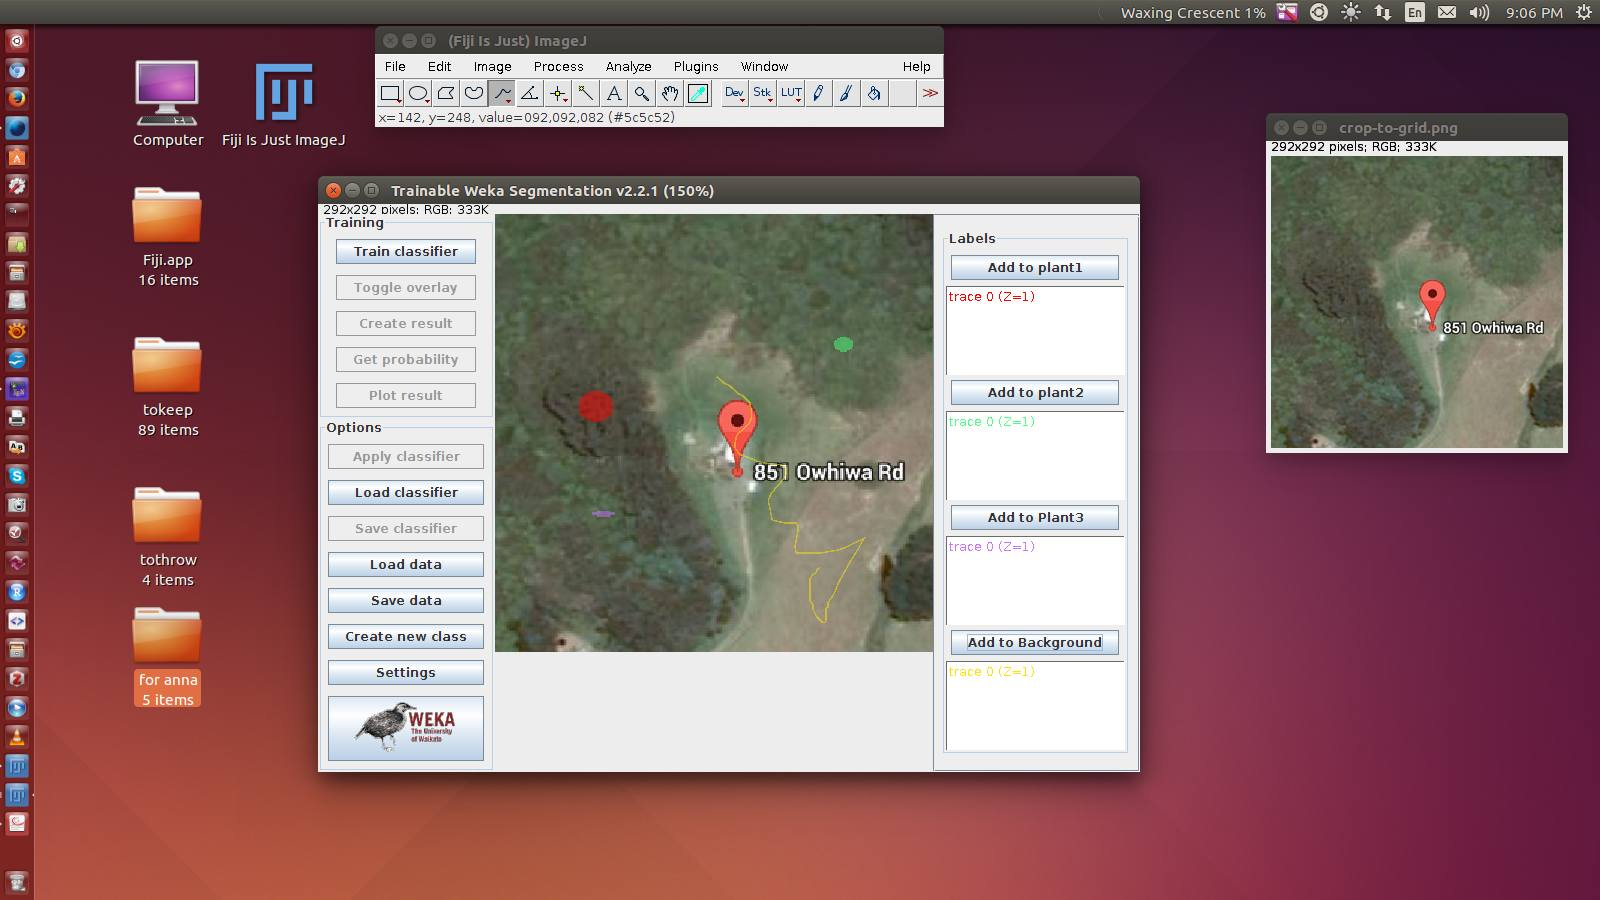
\includegraphics[width=0.7\linewidth]{../e-tws/5}
\caption{Add more categories if required. Use the ROI tools to add traces representing the target areas.}
\label{fig:5}
\end{figure}

\item Train the initial classifier.
\begin{figure}[htps!]
\centering
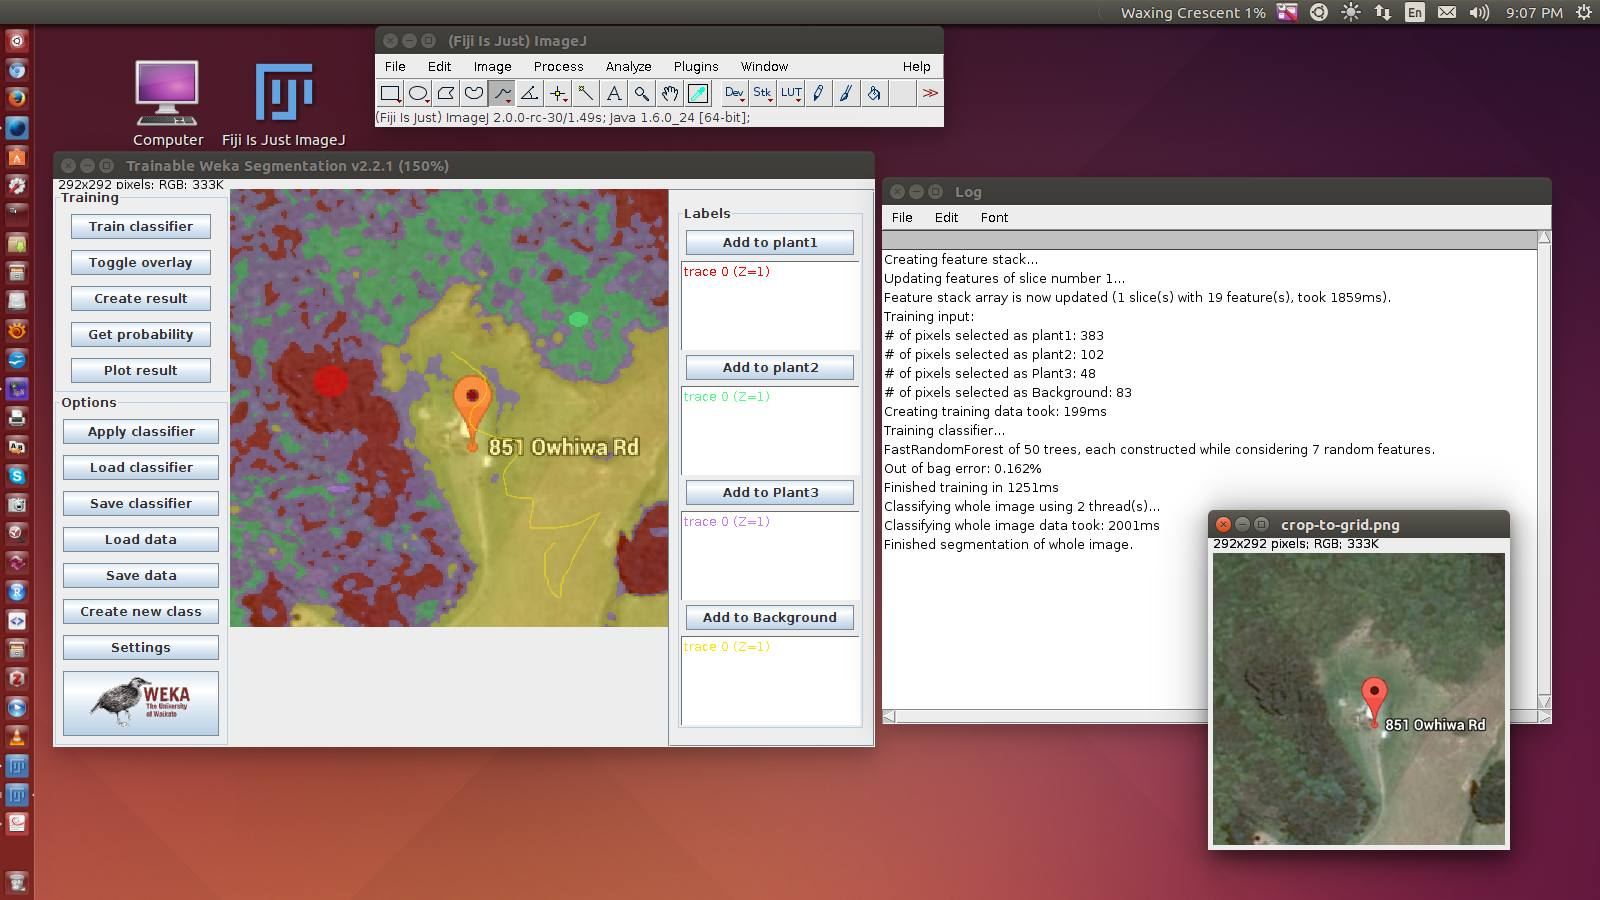
\includegraphics[width=0.7\linewidth]{../e-tws/6}
\caption{Initial classifier training and results.}
\label{fig:6}
\end{figure}

\clearpage

\item Check results and refine classifier.
\begin{figure}[htps!]
\centering
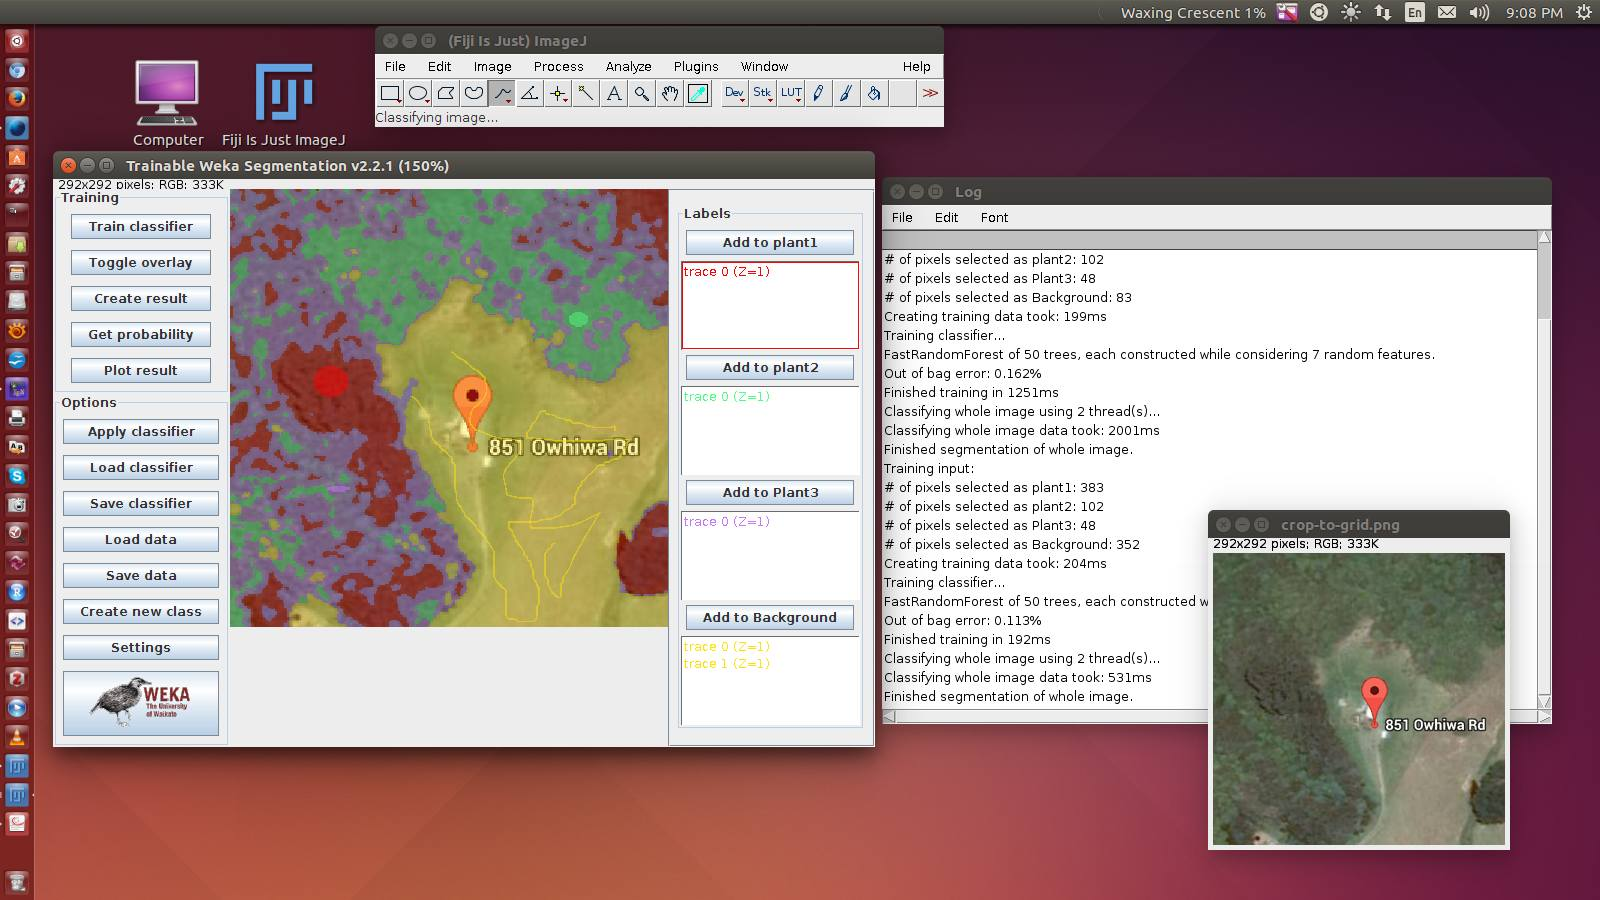
\includegraphics[width=0.7\linewidth]{../e-tws/7}
\caption{Final classifier training and results.}
\label{fig:7}
\end{figure} 

\item Save results - classified image, probability maps, data, model and log files (as per your folder set-up).

\begin{figure}[htps!]
\centering
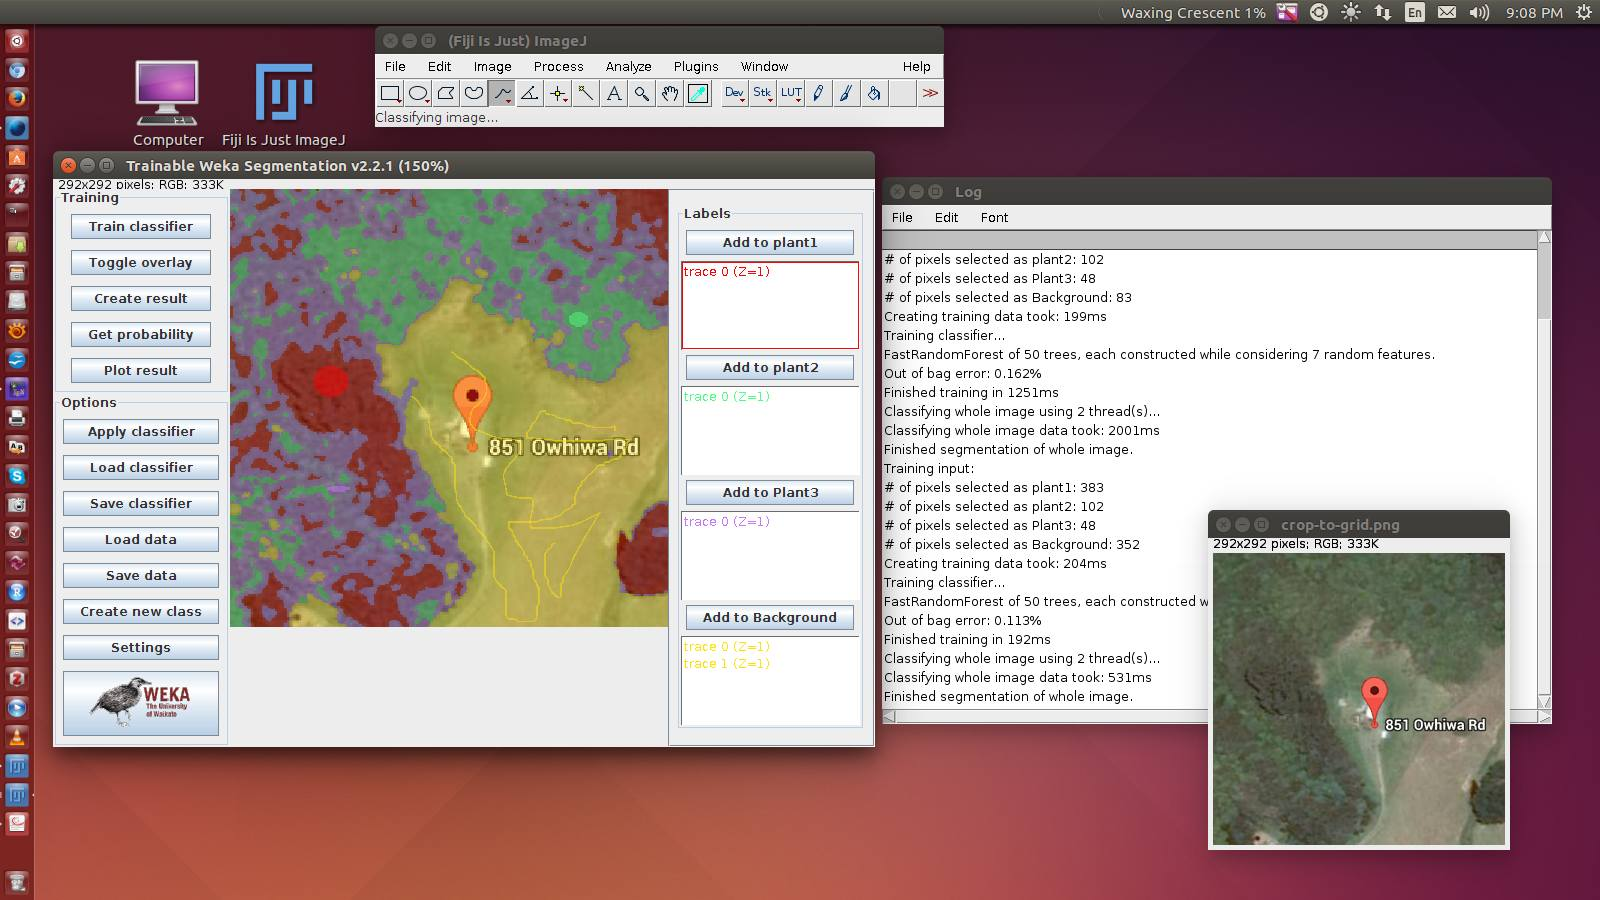
\includegraphics[width=0.7\linewidth]{../e-tws/7}
\caption{Save data.}
\label{fig:8}
\end{figure} 
\end{enumerate}

\section{Post-processing}
See FIJI or ImageJ sites for methods to quantify data from binary images. This step can be refined, 1) when your more sure about what you need, 2) and as you become more familiar with the techniques. I've included some literature that might be helpful.




\end{document}
